\documentclass[9pt]{extarticle}
\title{}
\author{Avinash Iyer}
\date{}
\usepackage[shortlabels]{enumitem}

%font setup
%
\usepackage{newpxtext,eulerpx}

%paper setup
\usepackage{geometry}
\geometry{letterpaper, portrait, margin=1in}
\usepackage{fancyhdr}

%symbols
\usepackage{amsmath}
\usepackage{mathtools}
\usepackage{amssymb}
\usepackage{hyperref}
\usepackage{gensymb}

\usepackage[T1]{fontenc}
\usepackage[utf8]{inputenc}

%chemistry stuff
\usepackage[version=4]{mhchem}
\usepackage{chemfig}

%plotting
\usepackage{pgfplots}
\usepackage{tikz}
\tikzset{middleweight/.style={pos = 0.5, fill=white}}
\tikzset{weight/.style={pos = 0.5, fill = white}}
\tikzset{lateweight/.style={pos = 0.75, fill = white}}
\tikzset{earlyweight/.style={pos = 0.25, fill=white}}

%\usepackage{natbib}

%graphics stuff
\usepackage{graphicx}
\graphicspath{ {./images/} }

%code stuff
%when using minted, make sure to add the -shell-escape flag
%you can use lstlisting if you don't want to use minted
%\usepackage{minted}
%\usemintedstyle{pastie}
%\newminted[javacode]{java}{frame=lines,framesep=2mm,linenos=true,fontsize=\footnotesize,tabsize=3,autogobble,}
%\newminted[cppcode]{cpp}{frame=lines,framesep=2mm,linenos=true,fontsize=\footnotesize,tabsize=3,autogobble,}

\usepackage{listings}
\usepackage{color}
\definecolor{dkgreen}{rgb}{0,0.6,0}
\definecolor{gray}{rgb}{0.5,0.5,0.5}
\definecolor{mauve}{rgb}{0.58,0,0.82}

\lstset{frame=tb,
	language=Java,
	aboveskip=3mm,
	belowskip=3mm,
	showstringspaces=false,
	columns=flexible,
	basicstyle={\small\ttfamily},
	numbers=none,
	numberstyle=\tiny\color{gray},
	keywordstyle=\color{blue},
	commentstyle=\color{dkgreen},
	stringstyle=\color{mauve},
	breaklines=true,
	breakatwhitespace=true,
	tabsize=3
}
% text + color boxes
\usepackage{tcolorbox}
\tcbuselibrary{breakable}
\newtcolorbox{problem}[1]{colback = white, title = {#1}, breakable}
\newtcolorbox{solution}{colback = white, colframe = black!75!white, title = Solution, breakable}
%including PDFs
\usepackage{pdfpages}
\setlength{\parindent}{0pt}

\pagestyle{fancy}
\fancyhf{}
\rhead{Ling Chen, Avinash Iyer, Nora Manukyan, Vincent Ng}
\lhead{Homework Section 3.3, Group}
\begin{document}{
  \begin{problem}{3.3.10}
    For every graph $G$, prove that $\beta(G) \leq \alpha'(G)$. For each $k\in \mathbb{N}$, construct a simple graph $G$ with $\alpha'(G) = k$ and $\beta(G) = 2k$.
    \tcblower
    Let $M$ be a matching with cardinality $\alpha'(G)$. Let $K$ be the set of vertices containing all the vertices in $M$ --- so, $K$ is of size $2\alpha'(G)$. We posit that $K$ is a vertex cover. Suppose toward contradiction that it were not. Then, there would exist $e=xy$ such that $e\in G$, $e\notin M$, and $x,y\notin K$. However, this would mean that $M$ would not be a maximum matching, as we would be able to add $e$ to it, which yields our desired contradiction. Since $K$ is a vertex cover, we know that the minimum vertex cover must be of size less than or equal to $K$. Therefore, we have that $\beta(G) \leq 2\alpha'(G)$.\\

    For every value of $k\in \mathbb{N}$, we can find a graph where $\alpha'(G) = k$ and $\beta(G) = 2k$ by using the disjoint union of $k$ copies of $C_3$.
  \end{problem}
  \begin{problem}{3.3.24}
    Let $G$ be a simple graph of even order $n$ with set $S$ of size $k$ such that $q(G-S) > k$. Prove that $G$ has at most ${k\choose 2} + k(n-k) + {n-2k-1 \choose 2}$ edges. Use this to determine the maximum size of a simple $n$-vertex graph with no $1$-factor.
    \tcblower
    We consider maximum values of the cardinality of the edge set within each subset. For the $k$ elements in $S$, we know that the maximum value of the edge size is ${k\choose 2}$. Additionally, for each of the $k$ vertices in $S$, there must be edges to the $n-k$ extra vertices (so as to create the components).\\

    Let $q(G-S) = \ell$. Then, to maximize the number of edges in $G-S$, we know that for $\sum n_i = n$, it is the case that $\sum {n_i\choose 2} \leq {n\choose 2}$. So, we know that maximizing the number of edges entails creating a clique of maximal size among the components of $G-S$. This means that $\ell-1$ odd components of $G-S$ are single vertices, and the final graph is $K_{(n-k)-(\ell-1)}$. To find the theoretical maximal size of this clique, we must minimize $(\ell-1)$ subject to the constraint that $\ell > k$ and $(n-k)-(\ell-1)$ is odd. The value that yields this result is $\ell = k+ 2$, meaning that our clique is $K_{n-2k-1}$, with size ${n-2k-1 \choose 2}$.\\

    Adding up all the edge sets, we get a final result of of maximum edge size of ${k\choose 2} + k(n-k) + {n-2k-1\choose 2}$.
  \end{problem}
  \begin{problem}{Tutte's Theorem}
    Do all the ``justifications'' in the proof of Tutte's Theorem.
    \tcblower
    \begin{description}[font=\scshape]
      \item[Necessity] The odd components of $G-S$ must have vertices matched to distinct vertices of $S$.
        \begin{description}
          \item[1.] Let $G-S$ be a graph with $q(G-S)$ odd components. Each of these components must contain at least \textit{one} unmatched vertex, each of which requires a distinct vertex in $S$ that was deleted. Thus, $q(G-S) \leq |S|$ is a necessary condition for $G$ to contain a $1$-factor.
        \end{description}
      \item[Sufficiency] When we add an edge joining two components of $G-S$, the number of odd components does not increase (odd and even together become odd, two edges of the same parity become even). Hence, Tutte's Condition is preserved by addition of edges.\\

        If $G' = G+e$ and $S\subseteq V$, then $q(G'-S)\leq q(G-S) \leq |S|$.
        \begin{description}
          \item[2.] If we were to add an edge between two odd components, then the new component will become even, thereby reducing the number of odd components. Otherwise, if we were to add an edge between two even components, then the new component will be even, keeping the number of components the same. Additionally, if 
            \begin{itemize}
              \item  If we were to add an edge between two odd components, then the new component will become even, thereby reducing the number of odd components.
              \item If we add an edge between an odd and an even component, then the new component is odd, keeping the number of odd components the same.
              \item If we were to add an edge between two even components, then the new component will be even, keeping the number of odd components the same. 
            \end{itemize}
            Therefore, since $G' = G + e$, we must have that $q(G'-S) \leq q(G-S)$, and we are assuming that $q(G-S) \leq |S|$, so $q(G'-S) \leq |S|$.
        \end{description}
        Also, if $G' = G + e$ has no $1$-factor, then $G$ has no $1$-factor.
        \begin{description}
          \item[3.] If $q(G'-S) > |S|$, which is our condition for finding a $1$-factor, and $q(G'-S) \leq q(G-S)$, then we know that $q(G-S) > |S|$.
        \end{description}
        Therefore, the theorem holds \textit{unless} there exists a simple graph $G$ such that $G$ satisfies Tutte's condition, $G$ has no $1$-factor, and adding any missing edge to $G$ yields a graph with a $1$-factor.
        \begin{description}
          \item[4.] If there exists no graph at $G$ that satisfies Tutte's condition and lacks a $1$-factor, then the theorem holds, as it proves that any graph that \textit{does} satisfy Tutte's condition \textit{must} contain a $1$-factor.\\

            We add as many edges to $G$ as possible without violating Tutte's condition and lacking a $1$-factor in such a way that adding an additional edge would yield a $1$-factor.
        \end{description}
        Let $G$ be a graph with the assumption. We will obtain a contradiction that $G$ does contain a $1$-factor.\\

        Let $U$ be the set of vertices in $G$ that have degree $|V|-1$ (i.e., the set of vertices in $G$ that are adjacent to every other vertex in $G$). We will prove via cases.
        \begin{description}[font=\normalfont\scshape]
          \item[Case 1: $G-U$ consists of disjoint complete graphs.] In this case, the vertices of the odd components in $G-U$ can be paired in any way with one extra vertex remaining in the odd components. Since $q(G-U) \leq |U|$ and each vertex of $U$ is adjacent to all of $G-U$, we can match the leftover vertices to the vertices of $U$.\\

            The remaining vertices are in $U$, which is a clique.
            \begin{description}
              \item[5.] The vertices of $U$, by construction, are adjacent to every other vertex in $G$, meaning that they are adjacent to every other vertex in $U$, so $U$ is a clique.
            \end{description}
            We have matched an even number of vertices in $G$ so far, so it suffices to show that $|V|$ is even. This follows by invoking Tutte's condition for $S = \emptyset$, since a graph of odd order would contain a component of odd order.
            \begin{description}
              \item[6.] If $G$ is a graph with odd order, it then has a component of odd order, so if $S = \emptyset$,  then $q(G-\emptyset) \geq 1 > |S| = 0$, which would mean Tutte's condition didn't hold.
              \item[7.]A sketch is shown below:\\
                \begin{center}
                  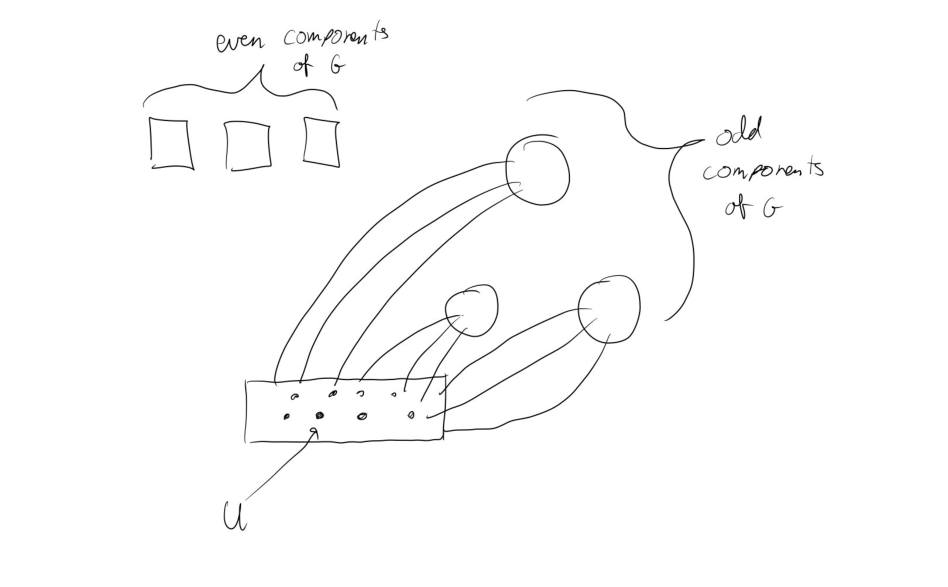
\includegraphics[width=10cm]{tutte_condition_sketch}
                \end{center}
            \end{description}
        \end{description}
      \item[Case 2: $G-U$ is not a disjoint union of cliques.] In this case, $G-U$ has two vertices at distance $2$; these are nonadjacent vertices $x,z$ with common neighbor $y\notin U$.
        \begin{description}
          \item[8.] WLOG, one of the components of $G-U$ is not a clique. Then, there is a vertex $x$ such that $x$ is not adjacent to $z$. Otherwise, $x\leftrightarrow z$ and the component would be complete. So, there must be a vertex $y$ such that $x\leftrightarrow y$ and $z\leftrightarrow y$. So, $d(x,z) = 2$.
        \end{description}
        Furthermore, $G-U$ has another vertex $w$ not adjacent to $y$, since $y\notin U$.
        \begin{description}
          \item[9.] It must be the case that $\exists w\in G-U$ such that $w\not\leftrightarrow y$. Else, if $y\leftrightarrow w$, then $y$ is adjacent to every vertex in $G-U$, which means $y\in U$, but since $y\notin U$, then it must be the case that $w\in G-U$ and $w\not\leftrightarrow y$.
        \end{description}
        By our choice of construction, we have that adding an edge to $G$ creates a $1$-factor. Let $M_1$ be the $1$-factor in $G + xz$, and let $M_2$ be the $1$-factor in $G + yw$. It suffices to show that $M_1 \triangle M_2 \cup \{xy,yz\}$ contains a $1$-factor avoiding $xz$ and $yw$, because this will be a $1$-factor in $G$.
        \begin{description}
          \item[10.] We know that the symmetric difference $F$ contains only the edges in $M_1$ or the edges in $M_2$ exclusively, and if we exclude any edges they have in common, as well as avoid both $xz$ and $yw$, then it will be a $1$-factor without any edges not in $G$.
        \end{description}
        Let $F = M_1\triangle M_2$. Since $xz \in M_1 - M_2$ and $yw \in M_2 - M_1$, both $xz$ and $yw$ are in $F$. Since every vertex of $G$ has degree $1$ in each of $M_1$ and $M_2$, every vertex of $G$ has degree $2$ or $0$ in $F$.
        \begin{description}
          \item[11.] Select an arbitrary vertex in $G$. It is either the case that $M_1$ and $M_2$ are incident on the vertex with unique edges, or they contain the same edge, in which case the edge is removed in the symmetric difference. Therefore every vertex has an even degree in $F$.
        \end{description}
        Hence, the components of $F$ are even cycles and isolated vertices. Let $C$ be the cycle of $F$ containing $xz$.\\

        If $C$ does not also contain $yw$, then the desired $1$-factor consists of the edges of $M_2$ from $C$ and all of $M_1$ not in $C$.
        \begin{description}
          \item[12.] By using the edges of $M_2$ in $C$, we avoid $xz$, and by using the edges of $yw$ outside of $C$, we avoid $yw$, and since $M_1$ and $M_2$ are $1$-factors, we know that this graph is a $1$-factor, and since it avoids $xz$ and $yw$, it is a $1$-factor in $G$.
        \end{description}
        If $C$ contains both $yw$ and $xz$, then to avoid them we use $yx$ or $yz$. In the portion of $C$ starting from $y$ along $yw$, we use the edges of $M_1$ to avoid using $yw$. When we reach either $x$ or $z$, we use $zy$ if we arrive at $z$, or else we use $yx$. In the remainder of $C$, we use the edges of $M_2$.
        \begin{description}
          \item[13.] Because we have already saturated either $x$ or $z$ in our current $1$-factor, we cannot use $M_1$ as it contains $xz$.
        \end{description}
        We have produced a $1$-factor of $C + \{xy,yz\}$ that does not use $xz$ or $yw$. Combined with $M_1$ or $M_2$ outside of $V(C)$, we create our desired $1$-factor.
    \end{description}
  \end{problem}
}\end{document}
